\begin{frame}[allowframebreaks]{Wasserstein GAN}
\begin{itemize}
    \item Wasserstein GAN uses wasserstein distance instead of crossentropy loss.
    \item Wasserstein distance that has a smoother gradient everywhere.
        \begin{figure}
            \centering
            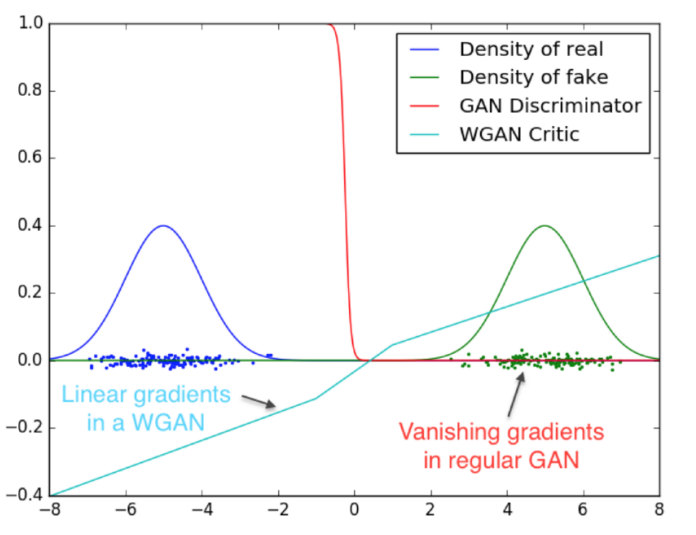
\includegraphics[height=0.6\textheight, width=\textwidth, keepaspectratio]{images/gan/wgan_1.png}
        \end{figure}
\end{itemize}
    
\end{frame}

\begin{frame}{Wasserstein Distance}
\begin{itemize}
    \item Intuitively, it is the shovels of earth moved to make two distributions look alike.
    \begin{figure}
        \centering
        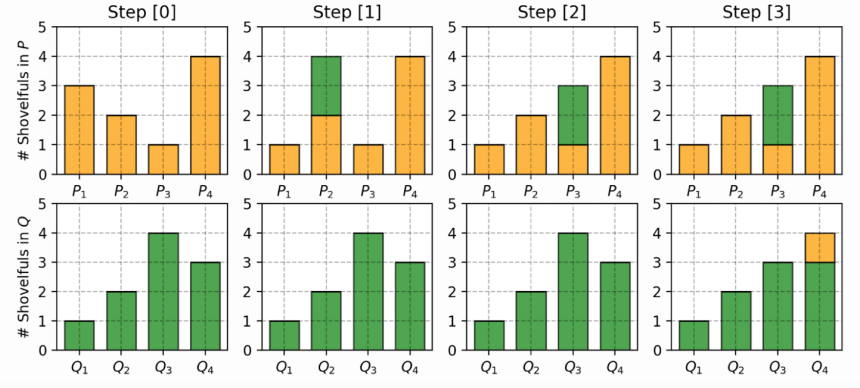
\includegraphics[height=0.6\textheight, width=\textwidth, keepaspectratio]{images/gan/wgan_2.png}
        \caption{Step by Step plan of moving dirt between piles $P$ and $Q$ to make them match}
    \end{figure}
    
\end{itemize}
    
\end{frame}

\begin{frame}[allowframebreaks]{WGAN}
\begin{figure}
    \centering
    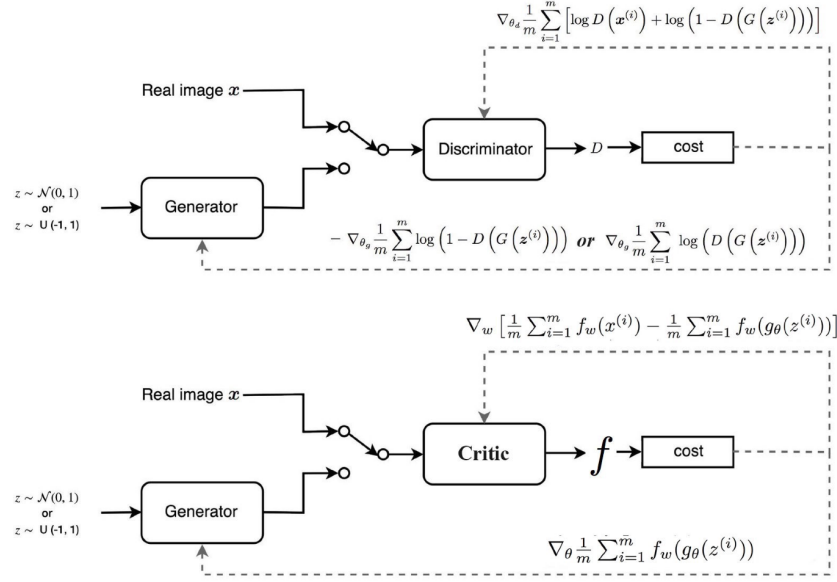
\includegraphics[height=0.9\textheight, width=\textwidth, keepaspectratio]{images/gan/wgan_3.png}
\end{figure}

\framebreak
\begin{figure}
    \centering
    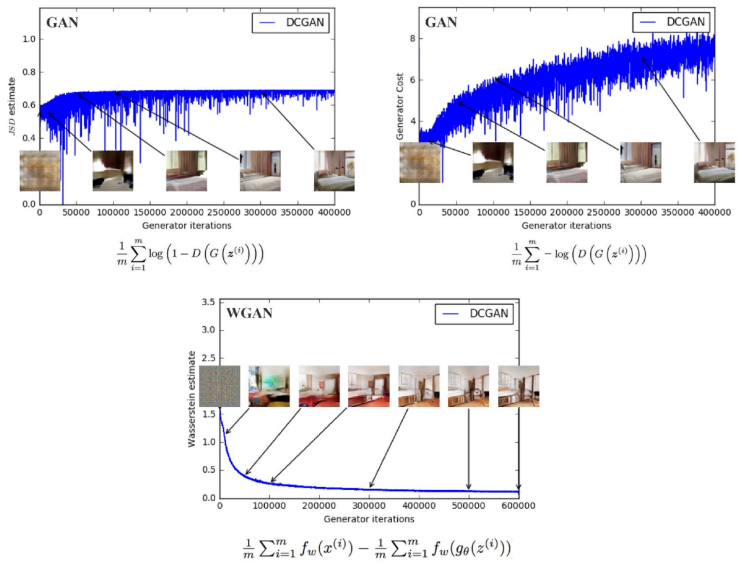
\includegraphics[height=0.9\textheight, width=\textwidth, keepaspectratio]{images/gan/wgan_4.png}
\end{figure}

\framebreak
\begin{figure}
    \centering
    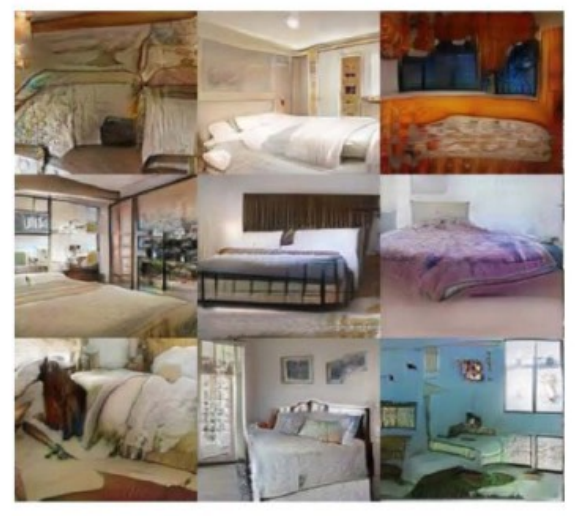
\includegraphics[height=0.8\textheight, width=\textwidth, keepaspectratio]{images/gan/wgan_5.png}
    \caption{WGAN generation results on bedroom images}
\end{figure}

\end{frame}